\documentclass[border=5pt]{standalone}
% Style commun aux figures de structure de MPMbox
% ------------------------------------------------
\usepackage[utf8]{inputenc}
\usepackage[T1]{fontenc}
\usepackage[english]{babel}
\usepackage{lmodern}
\usepackage{tikz}
\usetikzlibrary{positioning,arrows.meta,calc,fit,backgrounds,shapes.geometric}
% babel(french) rend « : » actif, ce qui casse les coordonnées polaires (90:4cm)
\usetikzlibrary{babel}

% pas de césure dans les boîtes étroites
\hyphenpenalty=10000
\exhyphenpenalty=10000
\tolerance=9999
\emergencystretch=3em

\definecolor{mpmBase}{HTML}{1F3A5F}    % classes de base
\definecolor{mpmBaseBg}{HTML}{E8EEF6}
\definecolor{mpmDeriv}{HTML}{4A7BA7}   % variantes
\definecolor{mpmDerivBg}{HTML}{F5F8FB}
\definecolor{mpmData}{HTML}{7A5230}    % données simulées
\definecolor{mpmDataBg}{HTML}{FBF3E8}
\definecolor{mpmAccent}{HTML}{A6432F}  % mise en avant (MPMxDEM)
\definecolor{mpmAccentBg}{HTML}{FBEEEB}
\definecolor{mpmGrey}{HTML}{5A6472}

\tikzset{
  base/.style={
    draw=mpmBase, line width=0.9pt, fill=mpmBaseBg, rounded corners=3pt,
    text width=#1, align=center, inner sep=6pt, font=\sffamily\small},
  base/.default=5.2cm,
  deriv/.style={
    draw=mpmDeriv, line width=0.6pt, fill=mpmDerivBg, rounded corners=2pt,
    text width=#1, align=left, inner sep=5pt, font=\sffamily\scriptsize},
  deriv/.default=7.4cm,
  data/.style={
    draw=mpmData, line width=0.7pt, fill=mpmDataBg, rounded corners=3pt,
    text width=#1, align=center, inner sep=5pt, font=\sffamily\scriptsize},
  data/.default=4.2cm,
  accent/.style={
    draw=mpmAccent, line width=0.8pt, fill=mpmAccentBg, rounded corners=2pt,
    text width=#1, align=left, inner sep=5pt, font=\sffamily\scriptsize},
  accent/.default=7.4cm,
  spine/.style={draw=mpmDeriv, line width=0.6pt},
  link/.style={draw=mpmGrey, line width=0.6pt, -{Stealth[length=4pt]}},
  dashlink/.style={draw=mpmGrey, line width=0.6pt, densely dashed,
                   -{Stealth[length=4pt]}, font=\sffamily\tiny},
  mpmcap/.style={font=\sffamily\scriptsize\itshape, text=mpmGrey},
}

% Titre d'une classe de base : \classname{Nom}{rôle}
\newcommand{\classname}[2]{{\bfseries #1}\\[2pt]{\scriptsize\itshape #2}}
% Ligne d'une variante : \variant{Nom}{description}
\newcommand{\variant}[2]{{\bfseries\ttfamily #1}\quad #2}

\begin{document}
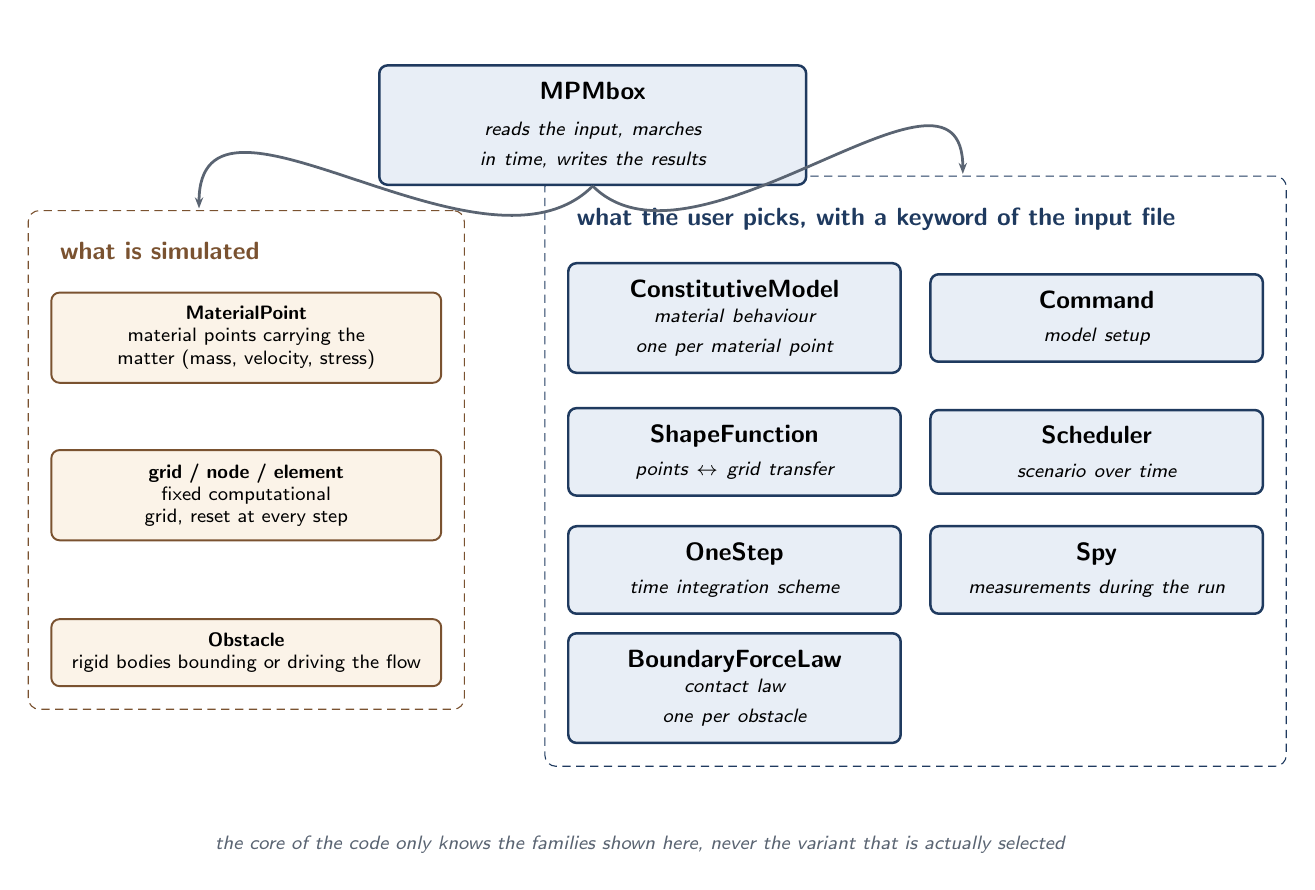
\begin{tikzpicture}

% ---- the conductor
\node[base=5.0cm] (BOX) at (1.0, 3.6)
  {\classname{MPMbox}{reads the input, marches in time, writes the results}};

% ---- what is simulated
\node[data=4.6cm] (MP)   at (-3.4, 0.9) {{\bfseries MaterialPoint}\\ material points carrying the matter (mass, velocity, stress)};
\node[data=4.6cm] (GRID) at (-3.4,-1.1) {{\bfseries grid / node / element}\\ fixed computational grid, reset at every step};
\node[data=4.6cm] (OBS)  at (-3.4,-3.1) {{\bfseries Obstacle}\\ rigid bodies bounding or driving the flow};

% ---- the interchangeable ingredients
\node[base=3.8cm] (CM)  at (2.8, 1.15) {{\bfseries ConstitutiveModel}\\[1pt]{\scriptsize\itshape material behaviour\\ one per material point}};
\node[base=3.8cm] (SF)  at (2.8,-0.55) {{\bfseries ShapeFunction}\\[1pt]{\scriptsize\itshape points $\leftrightarrow$ grid transfer}};
\node[base=3.8cm] (OS)  at (2.8,-2.05) {{\bfseries OneStep}\\[1pt]{\scriptsize\itshape time integration scheme}};
\node[base=3.8cm] (BFL) at (2.8,-3.55) {{\bfseries BoundaryForceLaw}\\[1pt]{\scriptsize\itshape contact law\\ one per obstacle}};

\node[base=3.8cm] (CMD) at (7.4, 1.15) {{\bfseries Command}\\[1pt]{\scriptsize\itshape model setup}};
\node[base=3.8cm] (SCH) at (7.4,-0.55) {{\bfseries Scheduler}\\[1pt]{\scriptsize\itshape scenario over time}};
\node[base=3.8cm] (SPY) at (7.4,-2.05) {{\bfseries Spy}\\[1pt]{\scriptsize\itshape measurements during the run}};
% ---- group titles (inside the frames)
\node[font=\sffamily\small\bfseries, text=mpmData, anchor=south west] (TD)
  at ($(MP.north west)+(0,0.28cm)$) {what is simulated};
\node[font=\sffamily\small\bfseries, text=mpmBase, anchor=south west] (TC)
  at ($(CM.north west)+(0,0.28cm)$) {what the user picks, with a keyword of the input file};

% ---- groups
\begin{scope}[on background layer]
  \node[draw=mpmData, densely dashed, rounded corners=4pt, inner sep=8pt,
        fit=(MP)(GRID)(OBS)(TD)] (GDATA) {};
  \node[draw=mpmBase, densely dashed, rounded corners=4pt, inner sep=8pt,
        fit=(CM)(BFL)(CMD)(SPY)(TC)] (GCHOIX) {};
\end{scope}

\draw[link, line width=1pt] (BOX.south) to[out=-135,in=90] ($(GDATA.north)+(-0.6cm,0.02cm)$);
\draw[link, line width=1pt] (BOX.south) to[out=-45,in=90] ($(GCHOIX.north)+(0.6cm,0.02cm)$);

\node[mpmcap, anchor=north, text width=13cm, align=center] at (1.6,-5.3)
  {the core of the code only knows the families shown here,
   never the variant that is actually selected};

\end{tikzpicture}
\end{document}
